\chapter{Proposta de Solução}
\label{cap:proposta}

A solucao proposta para permitir a realizacao de experimentos de plataformas de Cidades Inteligentes em ambientes emulados abrangendo diferentes cenarios em diferentes escalas sera
apresentada neste capitulo.
A discussao sobre os requisitos de uma possivel solucao para esse problema se dara de maneira generica, contudo, ao abordarmos a arquitetura, entraremos em alguns detalhes referentes ao
simulador e emulador de Cidades Inteligentes InterSCSimulator e a plataforma InterSCity, as ferramentas utilizadas neste trabalho.
Alem disso, serao apresentados alguns exemplos de implementacao de cenarios de Cidades Inteligentes seguindo a arquitetura proposta, trazendo em seguida os principais problemas e
dificuldades encontradas nesse processo.

\section{Requisitos da Solução}

Para a realizacao de experimentos em ambientes emulados de Cidades Inteligentes temos requisitos em diferentes niveis, desde a capacidade do emulador de representar o contexto
de uma cidade ate formas de comunicacao que permita a interacao entre o emulador e a plataforma de Cidades Inteligentes.
Portanto, dividimos os requisitos em requisitos de \textbf{fundamentais} e de \textbf{integracao}.

Para que uma ferramenta possa refletir o contexto de Cidades Inteligentes, onde o sensoriamento de diversos aspectos das cidades ja e uma realidade, e a atuacao (modificacao do estado
das cidades) segue uma crescente, consideramos que a mesma deva de alguma forma ter os conceitos abaixo representados:

\begin{itemize}
    \item \textit{Modelos aderentes a realidade de uma cidade}: a ferramenta deve implementar modelos que representem ao maximo a realidade de uma cidade, e nao apenas casos hipoteticos.
        Por exemplo, modelos de fluxo de automoveis nas vias devem incluir possiveis engarrafamentos.

    \item \textit{Execução em tempo real}: a dinamica da cidade deve ser emulada, ou seja, em tempo real. Essa dinamica representada nao deve ser executada nem mais rapida nem mais lenta do que
        aconteceria em um ambiente real de uma cidade.
        Esse e um requisito importante pois o desencadeamento de acoes nas cidades sao muitas vezes devido ao processamento de acoes acontecidas anteriormente, e as plataformas
        devem ter tempo habil para realizar tais acoes, como foi explicado nos capitulos anteriores.

    \item \textit{Geração de grande massa de dados}: para realizarmos experimentos realistas devemos ser capazes de gerar uma massa de dados na mesma escala de uma grande cidade por
        exemplo.
        Experimentos em escalas menores são úteis na validação de certos cenários, contudo não exercita uma plataforma de Cidades Inteligentes num contexto real, onde deverá
        interagir com milhões de sensores, atuadores e usuários.

    \item \textit{Comunicação em tempo de execução}: para que esse ambiente integrado seja viável, ambas as ferramentas devem ser capazes de se comunicarem em tempo de execução.
        Com isso, se torna possível a envio de dados de sensores e comandos de atuação durante a emulação.
\end{itemize}

Consideramos os pontos apresentados acima como \textbf{requisitos fundamentais}, sendo esses o minimo necessario para conseguirmos de fato representar um ambiente real de uma cidade.
Caso a ferramenta atenda os requisitos apresentados, se torna possivel a emulacao de cenários realistas no contexto de Cidades Inteligentes, podendo substituir \textit{testbeds}
reais, em uma escala maior, após a sua integração com a plataforma alvo.
Todavia, apenas essa emulacao nao viabiliza ainda a realizacao de experimentos com plataformas, ainda precisamos atender alguns \textbf{requisitos de integracao} entre o emulador
e a plataforma em questao.

Para termos um ambiente integrado precisamos definir um meio de comunicacao de duas vias, envio e recebimento de dados, em tempo real entre o emulador e a plataforma de Cidades Inteligentes.
Além disso, deve haver uma integração semântica que viabilize as ferramentas se comunicarem de maneira eficaz.
Abaixo sao apresentados os \textbf{requisitos de integracao} necessarios para obtermos um ambiente integrado de experimentacao para essas plataformas:

\begin{itemize}
    \item \textit{Integração semântica}: para que seja possível a comunicação em tempo de execução entre o emulador e a plataforma, ambos precisam entrar em um consenso semântico.
        Abaixo são apresentados os dois principais conceitos envolvidos e que acreditamos que seja necessário serem representados de alguma forma em ambas as ferramentas para que seja
        possível a integração.

        \begin{itemize}
            \item \textit{Recursos da cidade}: esse recursos da cidade, sendo eles qualquer coisa no contexto da cidade (automoveis, aparelhos publicos, vias e etc.), serao objetos tanto de
                sensoriamento e/ou atuacao por parte das plataformas de Cidades Inteligentes.

            \item \textit{Capacidades inerentes a cada recurso da cidade}: cada \textit{recurso da cidade} tem as suas respectivas capacidades, sendo elas de sensoriamento ou atuacao.
                Essas capacidades usualmente estão atreladas a dispositivos de IoT (\textit{Internet Of Things}) presentes nos recursos da cidade.
                Por exemplo, vagas de estacionamento podem ser monitoradas quanto a sua ocupacao, e semaforos de transito podem ter o seu estado modificado atraves de atuacao.
        \end{itemize}

    \item \textit{Envio de dados de sensoriamento em tempo real}: para que as funcionalidades relativas a coleta e armazenamento de dados, e processamento dos mesmos possam ser
        exercitadas pelas plataformas, precisamos enviar dados de todos os recursos presentes no cenario de experimentacao com tais capacidades em tempo real.
        Quanto maior for a escala do cenario de experimentacao mais dificil se torna essa tarefa, pois se faz necessario enviar milhoes de dados de sensores simultaneamente atraves
        do mesmo canal.
        Apesar de a demanda de tempo real poder se tornar um problema, ela se faz necessaria para que possamos chegar mais proximo de um cenario realista, onde recursos sensoriados
        da cidade poderao nao aguardar outros enviarem seus dados para enviar, apenas enviarao no tempo estipulado.

    \item \textit{Recebimento de dados de atucao em tempo real}: as plataformas, em dados cenarios de experimentacao, precisarao enviar comandos de atuacao para a cidade (neste caso,
        para o ambiente emulado) em tempo real.
        Diferente dos dados de sensoriamento, o fluxo de dados de atuacao e bem menor.
        Contudo, esse tipo de dado tem a sua propria peculiaridade, pois o emulador deve ser capaz de consumir essa dado em tempo de execucao e alterar o estado do ambiente emulado
        imediatamente.
        Isso porque ao modificar de alguma forma o estado do ambiente emulado influenciamos diretamente os dados de sensores naquele dado momento em diante, e os mesmos continuam
        sendo enviados para a plataforma em paralelo.
\end{itemize}

Portanto, acreditamos que ao termos um ambiente que atenda tanto os \textbf{requisitos fundamentais} quanto os de \textbf{integracao}, se torna possivel realizarmos experimentos
com plataformas de Cidades Inteligentes sem a necessidade de \textit{testbeds} reais.
Isso nos possibilita testar cenarios em escalas reais de uma cidade, alem de nos permitir emular cenarios que ainda nao sao passiveis de reproducao atraves de \textit{testbeds},
emulando tecnologias ainda nao existentes e cenarios futuristas.
Por exemplo, termos a possibilidade de emular um ambiente onde todos os carros da cidade sao autonomos se comunicando atraves de tecnologia \textit{5G}.

\section{Arquitetura}

Uma arquitetura de software foi desenhada visando atender principalmente os \textbf{requisitos de integração} para construção de um ambiente emulado de experimentação para plataformas
de Cidades Inteligentes, e será apresentada nesta seção.
A integração entre sistemas como apresentando no decorrer deste trabalho é uma tarefa complexa e demanda um projeto de software bem elaborado para que seja manutenível a longo prazo.
Neste trabalho integramos o emulador InterSCSimulator e a plataforma InterSCity para Cidades Inteligents, por isso, ambos serão detalhados quanto a sua respectiva arquitetura na
sequência, além de discutir como os \textbf{requisitos fundamentais e de integração} apresentados serão atendidos em cada ferramenta.

\subsection{Integração Emulador-Plataforma}

A integração entre emulador e plataforma de Cidades Inteligentes envolve principalmete a troca de dados em tempo de execução como foi apresentado neste capítulo.
Essa interação para envio e recebimento de dados a primeira vista simples, se torna complexa quando adicionamos a necessidade de resposta de ambas as partes em tempo real.
Por parte do emulador, a rápida reação ao receber um dado de atuação é essencial.
O recebimento desse dado acarretará um atualização no estado da emulação, que por sua vez terá impacto direto no pronto envio de dados de sensores que, por muitas vezes,
se dá de maneira temporizada.
Já para a plataforma, é necessária uma tomada de decisão ágil ao receber diferentes dados de sensores.
Os dados de sensores podem ser, por exemplo, utilizados como entrada para gatilhos de comandos de atuação e processamento em tempo real de eventos complexos.

Além desse desafio, enfrentamos também problemas de interoperabilidade entre o emulador e a plataforma.
Usualmente, os conceitos presentes no projeto de cada uma das ferramentas divergem, e essa camada de integração deve ser capaz de traduzir essa semântica para ambas as ferramentas.
Outro problema relacionado a interoperabilidade é a forma de transmissão desses dados, mais especificamente os protocolos de comunicação a serem utilizados.
Por exemplo, o emulador pode suportar apenas comunicação via protocolo AMQP e a plataforma prover uma API Restful e conexões via MQTT.
Mais uma vez, é papel da camada de integração tornar esse comunicação transparente para ambos os lados.

Tendo isso em vista, a arquitetura de integração adotada utiliza-se de um componente extra intermediando as duas ferramentas, emulador e plataforma, como pode ser visto na
FIGURA GERAL AQUITETURA.
Apesar de um componente extra adicionar complexidade e consequentemente aumentar o tempo gasto na transação desses dados, ele se faz necessário para solucionar os problemas
de interoperabilidade mencionados anteriormente.
Entretanto, ele deve ser o mais simples possível para que o acréscimo no tempo de envio e recebimento dos dados não aumente consideravelmente.
Portanto, utilizar ferramentas (emulador e plataforma) que se assemelhem conceitualmente e que compartilhem pilhas de protocolos de comunicação similares é o ideal,
facilitando o implementação de um ambiente integrado em conformidade com os requisitos apresentados inicialmente.

Na FIGURA GERAL ARQUITETURA, podemos ver os componentes presentes na arquitetura de integração do sistema aqui apresentada.
Como elucidado anteriormente, o componente de integração não pode possuir muitas responsabilidades, já que uma complexidade alta pode acarretar em um aumento expressivo no
tempo de transmissão dos dados, sendo esse um requisito importante para o sistema.
Já as ferramentas envolvidas, além de suas próprias funcionalidades, esperamos que as mesmas possuam um módulo de comunicação para suportar o fluxo de dados em tempo de execução.

O componente de integração tem a responsabilidade de solucionar os pontos mencionados anteriormente:

\begin{itemize}
    \item Tradução semântica entre o emulador e a plataforma

    \item Interoperação entre protocolos de rede

    \item Interferência mínima no tempo de envio e recebimento de dados
\end{itemize}

Como pode ser visto, o componente de integração tem como único objetivo atender requisitos não funcionais.
Ele deve tornar a comunicação do emulador e da plataforma transparente para ambos e adicionando a menor complexidade possível ao sistema.

Em resumo, devemos escolher ferramentas (emulador e plataforma) mais semelhantes possível, com o que diz respeito principalmente ao modelo conceitual e aos protocolos de
rede utilizados para comunicação; e implementar o componente de integração o mais simples possível, apenas com o objetivo de viabilizar a comunicação entre as ferramentas.

Para a validação da construção desse ambiente emulado de experimentação para plataformas de Cidades Inteligentes, usamos o emulador InterSCSimulator e a plataforma InterSCity,
sendo essas ferramentas desenvolvidas pelo nosso grupo de pesquisa. Ambas serão apresentadas a seguir, correlacionando os requisitos e a aquitetura de integração aqui
apresentadas.

\subsection{InterSCSimulator}

O InterSCSimulator é um simulador e emulador de código aberto baseado em agentes para Cidades Inteligentes que oferece uma interface simples para definição de
cenários de larga escala \cite{santana_17}.
Pelo fato da ferramenta ser configurável para execuação em modo de simulação ou de emulação, já atende um dos \textbf{requisitos fundamentais}.
Como apresentado nos capítulos anteriores, o diferencial da emulação é o fato de termos uma execução com uma noção de tempo real (um segundo de emulação é igual a
aproximadamente um segundo real) e permitir a interferência em tempo de execução por terceiros, sendo exatamente o que necessitamos para a construção desse
ambiente integrado de experimentação.

Para atingir a escalabilidade mencionada, o InterSCSimulator foi implementado usando a linguagem \textit{Erlang}.
Essa é uma linguagem funcional que visa facilitar a implementação de aplicações de larga escala, paralelas e distribuídas.
Algumas características herdadas do modelo de atores, que é implementado pelo \textit{Erlang}, são: paralelismo, execução distribuída, tolerância a falhas e
protocolo de comunicação \cite{santana_17}.
Essa escalabilidade é importante para que possamos atender o \textbf{requisito fundamental} que diz respeito a capacidade de geração de grandes massas de dados
para a plataforma.
O InterSCSimulator é capaz de emular/simular cenários com milhões de agentes executando simultaneamente, sendo possível emular cenários em uma escala realistas para
cidades de grande porte.

O InterSCSimulator foi implementado por Eduardo Zambom Santana, doutorando de nosso grupo de pesquisa, baseado no simulador de âmbito geral \textit{Sim-Diasca}.
A Figura \ref{fig:simulator_architecture} apresenta a sua arquitetura, onde, em azul, estão os diferentes tipos de agentes que podem existir no ambiente
emulado/simulado e, em vermelho, a definição dos cenários de Cidades Inteligentes, tudo isso sendo executado no topo do simulador \textit{Sim-Diasca}.

%\begin{figure}[ht]
%	\centering
%	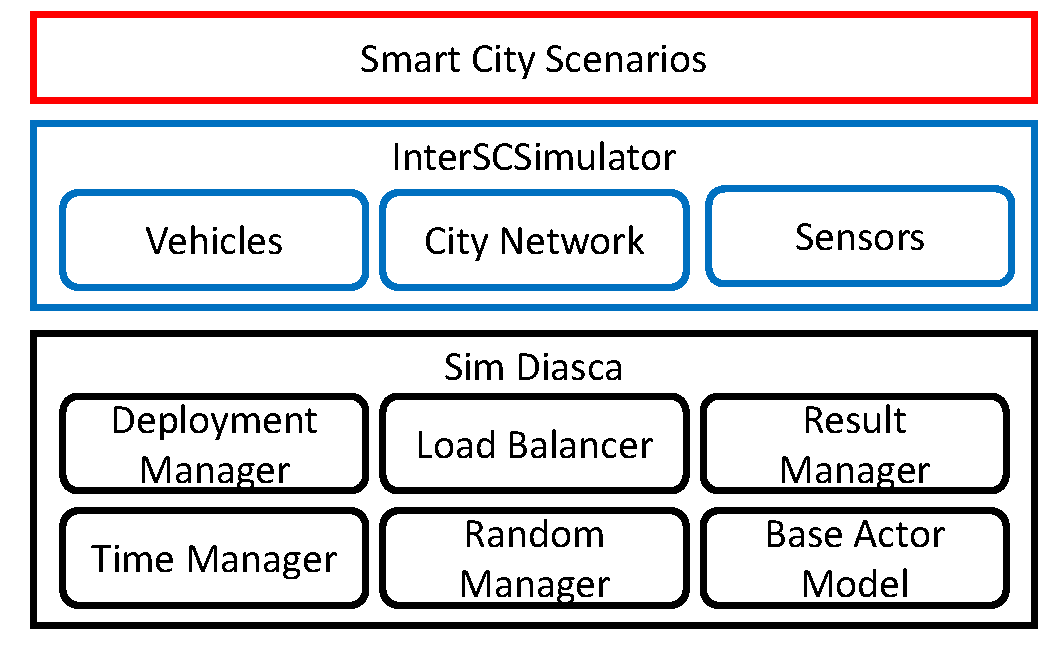
\includegraphics[width=0.5\textwidth]{figures/Arquitetura.pdf}
%	\caption{Arquitetura do InterSCSimulator}
%	\label{fig:simulator_architecture}
%\end{figure}

Fazendo um paralelo com um dos \textbf{requisito de integração} listados neste capítulo, cada \textit{Recurso} da cidade pode ser modelado como um agente da emulação/simulação.
Ou seja, um carro, uma vaga de estacionamento ou um ponto de parada de ônibus serão representados como agentes (caixas azuis na Figura \ref{fig:simulator_architecture})
na arquitetura do InterSCSimulator.
Na definição desses agentes especificamos o seu comportamento a cada passo da emulação/simulação.
Com isso, podemos especificar quais as \textit{Capacidades} de cada agente e adotar modelos aderentes com a realidade das cidades modernas.
O interessante dessa arquitetura baseada em agentes é o fato da implementação dos mesmos terem um grau de independência muito grande, onde é preciso apenas a definição
das mensagens que serão trocadas em tempo de execução.

Além disso, no contexto deste trabalho, foi adicionado um novo elemento a arquitetura da ferramenta para troca de dados com sistemas externos,
sendo esse um dos \textbf{requisitos fundamentais e de integração} para obtermos um ambiente realista de experimentação.
Esse novo elemento nada mais é do que um novo agente onde o seu papel é receber e enviar mensagens de sensores e atuadores, seja no contexto de outros agentes ou de
outros sistemas.

Na implementação de um agente do InterSCSimulator podemos definir diversos comportamentos em diferentes momentos do seu cliclo de vida.
Podemos especificar o que será feito durante a sua criação, a sua destruição, a sua primeira ação na emulação/simulação e durante cada ciclo de execução.
Com isso, condições e caminhos dependentes do estado da emulação/simulação podem ser definidos para cada um dos tipos de agentes, flexibilizando a implementação dos
mais diversos modelos e formas de prover suas capacidades.
Essa liberdade para implementação de diversos comportamentos dos agentes nos permite usar modelos realistas e viabilizar as capacidades dos recursos no contexto das cidades,
atendendo mais um \textbf{requisito fundamental} e outro de \textbf{integração}.
Por exemplo, um carro após a sua partida em direção ao seu destino, calcula a cada ciclo de execução o fluxo de carros na via em que se encontra para o calculo da
sua velocidade naquele instante, além de publicar a seu atual posição.
Nesse caso, podemos utilizar os mais diversos modelos matemáticos para calcular o fluxo de carros ou para determinar a sua velocidade, ao passo que a sua capacidade
de publicar sua localização georreferenciada também é atendida.

Na Figura \ref{fig:simulator_components}, são apresentados os componentes do simulador.
Inicialmente são passadas entradas para a emulação/simulação (arquivos XML) que em conjunto formam o cenário a ser emulado/simulado, esse cenário é executado e a
saída é criada com todos os eventos ocorridos na emulação/simulação.
A partir dessa saída existe a possibilidade de geração de uma visualização em um mapa ou através de gráficos.

%\begin{figure}[ht]
%	\centering
%	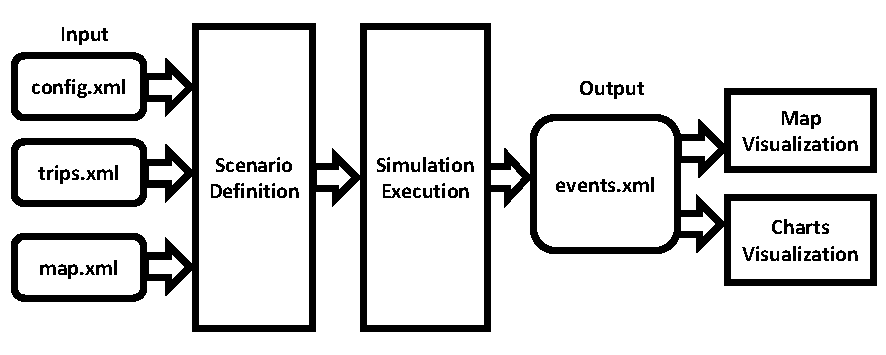
\includegraphics[width=0.7\textwidth]{figures/Components.pdf}
%	\caption{Componentes do InterSCSimulator}
%	\label{fig:simulator_components}
%\end{figure}

Como entrada, o InterSCSimulator recebe três arquivos XML. O \textit{config.xml} contém parâmetros da emulação/simulação, sendo eles o tempo total, o formato do
arquivo de saída e o caminho para o diretório contendo os outros arquivos de entrada e para geração do arquivo de saída.
O grafo representando a infraestrutura rodoviária da cidade é descrito no arquivo \textit{map.xml}, nesse grafo as vias são correspondentes as arestas e as esquinas entre
duas ou mais vias aos nós.
E por fim, as viagens a serem executadas são especificadas no arquivo \textit{trips.xml}, cada viagem contendo o seu tempo de início, modo de transporte, origem e destino.
Todas as ações realizadas pelos agentes são salvos no arquivo \textit{output.xml}, podendo haver quatro ações possíveis: 1) início de viagem, 2) saída de uma via,
3) entrada em uma via, e 4) chegada ao destino final.
O tempo, a localização e o modo de transporte utilizado pelo agente são registrados quando essas ações são salvas.

No trabalho desenvolvido por Eduardo Zambom Santana foi desenvolvido um emulador e simulador de larga escala, que já foi capaz de simular mais de 4 milhões de
agentes se movendo pela cidade de São Paulo~\cite{santana_17}.
Os modos de transportes suportados até então são carro, ônibus, metrô e a pé.
Neste trabalho além de melhorias feitas nos modelos existentes, novos agentes forma adicionados a simulação, além de agora ser possível a publicação e recebimento de
eventos em tempo de execução de maneira assícrona.

\subsection{Plataforma InterSCity}

A plataforma InterSCity é um projeto de código aberto, baseado em microsserviços que visa permitir a pesquisa colaborativa, desenvolvimento e experimentos em Cidades
Inteligentes~\cite{arthur_17}.
A plataforma foi desenvolvida baseada em uma arquitetura de referência para plataformas de Cidades Inteligentes~\cite{santana_2016}, ela provê um conjunto de serviços
alto-nível baseado em nuvem para gerenciar recursos de \textit{IoT} heterogêneos~\cite{arthur_17}.

O projeto InterSCity visa atacar dois dos principais problemas arquiteturais no desenvolvimento de uma plataforma de alta qualidade que possa ser usada na prática no
contexto de Cidades Inteligentes: escalabilidade e evolução do software~\cite{arthur_17}.
Escalabilidade é necessária pelo fato da plataforma ter que interagir com um grande número de dispositivos \textit{IoT} espalhados pela cidade, milhões de usuários e
um grande tráfego de dados.
Como as cidades mudam constantemente, a questão da evolução é essencial, já que requisitos podem surgir ou mudar a qualquer momento, e adaptar a plataforma a fim de
incorporar novas funcionalidades não deve ser um empecilho.
Para resolver esses dois problemas apresentados, foram adotadas as seguintes estratégias~\cite{arthur_17}:

\begin{itemize}
	\item Modularidade via microsserviços
	\item Modelos e dados distribuídos
	\item Evolução descentralizada
	\item Reuso de projetos de software livre
	\item Adoção de padrões abertos
	\item Comunicação síncrona e assíncrona
	\item Serviços livres de estado
\end{itemize}

A Figura \ref{fig:platform_architecture} apresenta a arquitetura da plataforma InterSCSity.
Atualmente, ela é composta de 6 microsserviços:
\textit{Resource Adaptor}, oferece uma abstração para comunicação com os dispositivos \textit{IoT};
\textit{Data Collector}, responsável por coletar os dados dos sensores conectados;
\textit{Actuator Controller}, oferece uma interface para atuação junto aos dispositivos de \textit{IoT} com tais capacidades;
\textit{Resource Catalog}, possui dados estáticos dos recursos da cidade cadastrados;
\textit{Resource discovery}, provê um serviço de descoberta de recursos;
e \textit{Resource Viewer}, disponibiliza uma visualização simples dos recursos da cidade. 

%\begin{figure}[ht]
%	\centering
%	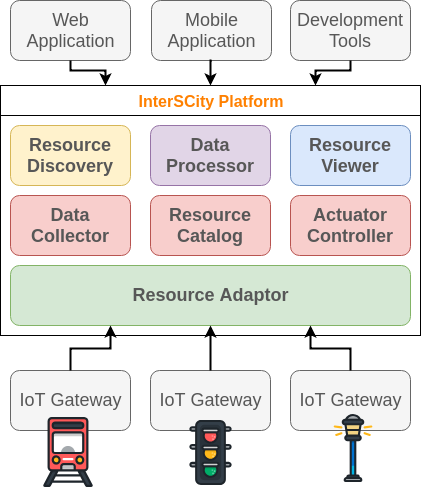
\includegraphics[width=0.5\textwidth]{figures/platform_architecture.png}
%	\caption{Arquitetura da plataforma InterSCity}
%	\label{fig:platform_architecture}
%\end{figure}

A comunicação entre esses microsserviços pode se dar de maneira síncrona ou assíncrona dependendo da situação.
A comunicação síncrona é feita via API \textit{Restful}, ou seja, requisições HTTP; e a assíncrona se dá via RabbitMQ, uma implementação do protocolo AMQP.
O objetivo do protocolo AMQP é criar um padrão aberto para troca de mensagens assíncronas interoperável e de larga escala~\cite{vinoski_2006}.
A principal vantagem desse protocolo é permitir que o \textit{broker} de mensagens tome as decisões de roteamento, não necessitando a aplicação ter conhecimento
desse processo~\cite{vinoski_2006}.

A plataforma traz uma abstração chamada \textit{Resource}, que representa um recurso real da cidade, como ônibus, hospital, paradas de ônibus.
Cada um desses \textit{Resources} possuem \textit{Capabilities}, que pode ser de sensoriamento ou atuação, usualmente vinculados a algum tipo dispositivo \textit{IoT},
como capacidade de medir temperatura ou capacidade de mudar o estado de um semáforo.
Esses conceitos são os mesmos apresentados como requisitos para a construção de um ambiente integrado de experimentação para Cidades Inteligentes.
Como apresentado na seção anterior, semânticamente, esses recursos e capacidades aqui apresentados estarão associados a agentes e a definição de ações durante o seu
ciclo de vida no InterSCSimulator.

Na seção a seguir serão apresentados alguns exemplos de implementação da arquitetura aqui proposta utilizando o emulador InterSCSimulator e a plataforma InterSCity
para Cidades Inteligentes.

\section{Exemplos de Implementação}

Com o intuito de validar a arquitetura proposta foram implementados dois cenários de Cidades Inteligentes no ambiente integrado de experimentação.
Priorizamos implementar cenários de experimentação onde pudéssemos explorar todos os requisitos apresentados neste capítulo.

No primeiro cenário realizamos experimentos no contexto de um estacionamento inteligente (conhecido com \textit{Smart Parking}), onde carros circulam pela cidade e ao
final do seu percurso procuram por uma vaga de estacionamento disponível mais próxima do seu destino, utilizando-se da plataforma para isso.
Nesse cenário, incluímos um novo agente à emulação e implementamos um mecanismo para publicação dos eventos ocorridos e requisição a serviços da plataforma em tempo real
e de forma assíncrona.

O segundo cenário de experimentação envolve a melhoria do fluxo de carros através da utilização de Placas de Mensagens Variadas (PMVs) espalhadas pela cidade.
Nesse cenário a plataforma identifica trechos de maior trânsito e atua na cidade atualizando as mensagens apresentadas pelas PMVs em tempo real, notificando os
motoristas da lentidão no trecho, que por sua vez podem recalcular a sua rota evitando congestionamentos.
Para viabilizar esse experimento nos utilizamos das melhorias implementados no primeiro cenário, modificamos o modelo de trânsito para melhor se adequar a realidade e
implementamos o mecanismo de recebimento de comandos de atuação em tempo de execução.

Cada um desses cenários serão apresentados nas seções a seguir, de maneira a exemplificar a implementação da arquitetura proposta através da utilização do emulador
InterSCSimulator a a plataforma InterSCity para Cidades Inteligentes.

\section{Estacionamento Inteligente}

Como foi apresentado, neste cenário de experimentação, emulamos um motorista realizando o seu percurso de carro e ao final procurando uma vaga disponível mais próxima ao
seu destino, provavelmente utilizando um aplicativo móvel que se comunica com a plataforma InterSCity.
Trazendo os conceitos de recursos da cidade e capacidades para esse cenário, temos os carros e as vagas de estacionamento sendo recursos, onde os carros são capazes de
fornecer a sua geolocalização (por exemplo via GPS) e as vagas de fornecer informação quanto a sua disponibilidade (por exemplo através de sensores infravermelho e uma
redes de sensores).

Esse cenário foi definido com o intuito de realizar experimentos envolvendo o serviço de descoberta de recursos da plataforma InterSCity.
Portanto, o aplicativo enviaria a posição do carro naquele momento, o seu destino final e o raio de busca, e a plataforma traria uma lista de vagas de estacionamento
disponíveis mais próximas.
Já no InterSCSimulator, foi necessário realizar algumas melhorias para que os \textbf{requisitos de emulação} fossem atendidos.
Um novo agente para gerenciar as vagas de estacionamento da cidade, chamado \textit{Parking Controller}, foi implementado.
Esse agente possui a responsabilidade de gerenciar e armazenar dados referentes as vagas de estacionamento, e fazer a interface de comunicação com o componente de
integração que será apresentado mais adiante.
Além disso, modificamos o modelo de viagem do agente \textit{Carro}.
Anteriormente, o \textit{Carro} saia de uma origem e percorriar o seu trajeto até o destino, agora ao chegar próximo do seu destino ele requisita uma vaga disponível mais
próxima e se dirige até a mesma.
Com essas melhorias pudemos emular um cenário que se aproxima da realidade.

Para ilustrar o modelo descrito, a seguir será apresentado o ciclo de emulação de um agente \textit{Carro} neste cenário:

\begin{enumerate}
    \item O agente \textit{Carro} é criado

    \item O caminho mais curto entre a origem e o destino é calculado

    \item O agente parte da sua origem no tempo determinado

    \item Ao chegar no nó anterior ao seu destino, uma vaga de estacionamento disponível é requisitada ao agente \textit{Parking Controller}

    \item Ao receber a vaga de estacionamento, o seu trajeto é recalculado em direção a mesma

    \item O agente se direciona e estaciona na vaga de estacionamento descoberta 
\end{enumerate}

Um fluxo alternativo a essa execução seria o carro modificar o seu percurso em direção da vaga de estacionamento (disponível até então), e ao chegar nela outro
carro a ter ocupado antes, sendo esse um caso comum nas grandes cidades.
Nesse caso, outra vaga de estacionamento é requisitada aumentando o seu raio de busca com o intuito de sempre encontrar vagas disponíveis.

Quando o agente \textit{Carro} por fim estaciona em uma vaga disponível, o agente \textit{Parking Controller} é notificado e atualiza a sua estrutura de dados indicando
que a vaga foi ocupada pelo carro.
Além do mais, esse agente é responsável por atualizar o estado da vaga de estacionamento na plataforma.

Agora pensando nos \textbf{requisitos de integração}, o emulador precisa requisitar a plataforma em busca de vagas disponíveis mais próximas, e atualizar o estado
das vagas de estacionamento.
A plataforma InterSCity provê um \textit{API Restful} para comunicação com seus serviços (como o de descoberta de recursos), e o estado dos seus recursos podem ser
atualizados através da própria API ou via protocolo AMQP (\textit{Advanced Message Queuing Protocol}).
O AMQP é um protocolo de troca de mensagens assíncronas que visa a escalabilidade e a interoperabilidade \cite{Vin06}.
Esse levantamento é importante para a tomada de decisão de quais as responsabilidades e como será implementado o componente de integração.
Tendo em vista que a complexidade do componente de integração deve ser a menor possível, e a não existência de um meio de publicação de eventos em tempo de execução
no InterSCSimulator, decidimos utilizar o RabbitMQ (implementação do protocolo AMQP) na implementação desse novo meio de comunicação.
Com isso, o emulador poderia atualizar o estado das vagas diretamente na plataforma de forma assíncrona, sem necessidade de auxílio do componente de integração.
As requisições HTTP feitas ao serviço de descoberta da plataforma seriam feitas pelo componente de integração, principalmente pelo fato de requisições HTTP serem
síncronas, o que poderia travar a emulação na espera por uma resposta.

Para facilitar o entendimento da integração realizada, dividiremos a explicação em duas partes: a primeira visando a requisição de vagas disponíveis mais próximas
do carro ao serviço de descoberta da plataforma InterSCity; e a segunda apresentado o fluxo de atualização do estado de uma vaga de estacionamento (ocupada
ou disponível) baseada na emulação.

A Figura \ref{fig:descoberta} apresenta a integração realizada para utilização do serviço de descoberta provido pela plataforma InterSCity.
O componente de integração foi chamado de \textit{Parking Spot Discoverer}, e foi implementado como um agente Erlang que consegue se comunicar com os agentes da
simulação via troca de mensagens.
O uso do componente de integração se fez necessário para que a emulação exerça a carga que aplicações exerceriam utilizando o protocolo HTTP para acessar
a \textit{API Restful}.
Como dito, requisições HTTP são síncronas, e a realização das mesmas dentro da emulação atrasaria consideravelmente a sua finalização, já que bloquearia a
execução dos agentes enquanto aguardariam a resposta da plataforma.
Antes de chegarmos a tal solução implementamos uma versão onde o próprio emulador realizava requisições HTTP para a plataforma em tempo de execução, entretanto,
essa solução gerou um enorme gargalo.
Descrevemos abaixo o fluxo de atividades apresentado na Figura \ref{fig:descoberta}.

\begin{enumerate}
    \item Ao chegar um nó antes do seu destino, o \textit{Car} solicita a vaga de estacionamento para o agente \textit{Parking Controller}, passando a sua
	localização como parâmetro.

	\item O agente \textit{Parking Controller} então envia a localização para o \textit{Parking Spot Discoverer} que solicita a vaga disponível mais próxima,
	em um raio de 500 metros.

	\item O \textit{Parking Spot Discoverer} faz uma requisição HTTP para o serviço de descoberta da plataforma que retorna a vaga em questão.
	Caso não seja encontrada uma vaga disponível (não ocupada) em um raio de 500 metros, esse raio é multiplicado por dois até que se encontre uma vaga
	disponível.

	\item O identificador da vaga é retornado para o agente \textit{Parking Controller} e ele marca a vaga como utilizada em uma estrutura de dados mantida no emulador.

    \item O identificador da vaga é recebido pelo agente \textit{Car} e a rota é recalculada para chegar até ela.
\end{enumerate}

%\begin{figure}[ht]
%	\centering
%	\includegraphics[width=\textwidth]{figures/integration_get_data.png}
%	\caption{Integração para descoberta de vagas livres próximo do destino da
%	viagem}
%	\label{fig:descoberta}
%\end{figure}

A Figura \ref{fig:atualizacao} apresenta a integração realizada com o intuito de atualizar o estado das vagas de estacionamento na plataforma baseado nos
acontecimentos da emulação.
Como foi adicionado a funcionalidade de publicação dos eventos da emulação via RabbitMQ para os interessados, não foi necesário a utilização do
componente de integração, já que a plataforma também utiliza o mesmo protocolo para divulgação dos seus dados entre microsserviços.
O fluxo apresentado na Figura \ref{fig:atualizacao} contém os seguintes passos.

\begin{enumerate}
    \item O agente \textit{Car} estaciona na vaga de estacionamento e notifica o \textit{Parking Controller}.

	\item O \textit{Parking Controller} informa, via \textit{RabbitMQ}, que a vaga está ocupada usando o seu identificador.

	\item O \textit{RabbitMQ} repassa esse dado para os microsserviços \textit{Resource Catalog} e \textit{Data Collector}.
\end{enumerate}

%\begin{figure}[ht]
%	\centering
%	\includegraphics[width=\textwidth]{figures/integration_publish_data.png}
%	\caption{Integração para publicar dados}
%	\label{fig:atualizacao}
%\end{figure}

Vale ressaltar que as atividades 2 e 3 apresentadas na Figura \ref{fig:atualizacao} também são executadas quando a vaga é liberada.
Após dez minutos que o agente está estacionado na vaga, o agente \textit{Parking Controller} libera a vaga na estrutura de dados mantida dentro do simulador e informa o
ocorrido para a plataforma.
Com isso, a plataforma atualiza os dados da vaga tanto quando ela é ocupada quando liberada.

Após a implementação da arquitetura descrita, fomos capazes de executar experimentos de larga escala no contexto de estacionamento inteligente.
Os resultados obtidos serão apresentados no próximo capítulo.

Todavia, não exercitamos todos os requisitos apresentados para a construção de um ambiente emulado e integrado para experimentação de plataformas de Cidades Inteligentes.
Por isso, implementamos um segundo cenário de Cidades Inteligentes onde, por exemplo, a atuação na cidade se fez necessária.


\section{Melhoria do Fluxo de Carros através de PMVs}

\section{Problemas e Dificuldades}
